\documentclass[a4paper, oneside]{article}
\usepackage[T1]{fontenc}
\usepackage[utf8]{inputenc}
\usepackage[english]{babel}
\usepackage{frontespizio}
\usepackage{graphicx}
\usepackage{listings}
\usepackage{scrextend}
\usepackage[margin=1.2in]{geometry}
\usepackage[font=small,labelfont=bf]{caption}
\usepackage{url}
\usepackage{hyperref}
\usepackage{verbatim}
\usepackage{xcolor}

\begin{document}
\selectlanguage{english}
\baselineskip 13pt
\hypersetup{
    colorlinks=true,
    linkcolor=blue,
}

% ---- FRONTESPIZIO ----- 
\begin{frontespizio} 
\Preambolo{\renewcommand{\frontpretitlefont}{\fontsize{15}{12}\scshape}}
\Istituzione {University of Pisa}
\Divisione {Scuola di Ingegneria}
\Corso [Laurea]{Artificial Intelligence and Data Engineering}
\Annoaccademico {2019--2020}
\Titolo {Task2 documentation}
\Filigrana [height=4cm,before=0.28,after=1]{./images/stemma_unipi.png}
\Rientro {1cm}
\Candidato {Giacomo Mantovani}
\Candidato {Stefano Poleggi}
\Relatore {Prof. Pietro Ducange}
 \Punteggiatura {}
\end{frontespizio}


\clearpage


% ----- INDICE -----
	\tableofcontents\thispagestyle{empty}
	\clearpage


\section{Introduction}\pagenumbering{arabic}
The \textbf{TweetQuake} application offers a real-time earthquake detection service in Italy. When the application opens up it will start fetching tweets and analyzing them to recognize ones related to an earthquake.
The application will show the number of tweets analyzed so far and the corresponding number of earthquake tweets and non-earthquake tweets. When some earthquake tweets are recognized the application show a warning message, if there is a trend of earthquake tweets then the application will show an emergency message. If the button at the end of the page is clicked then a new window containing the last recognized earthquakes opens up.
\vspace{5mm}
\begin{figure}[h]
\centering
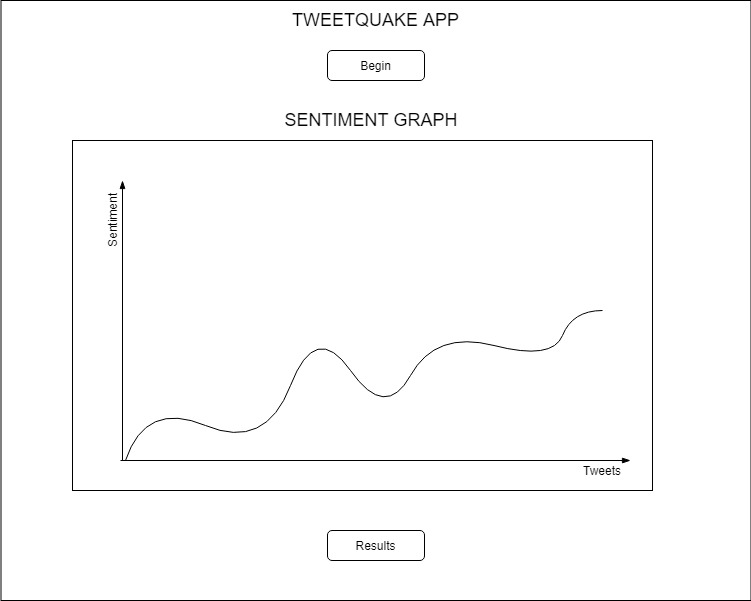
\includegraphics[width=\textwidth]{./images/diagrams/HomeMockup} 
\caption{Home Page Mockup}
\label{fig:mockup}
\end{figure}

\begin{figure}[h]
\centering
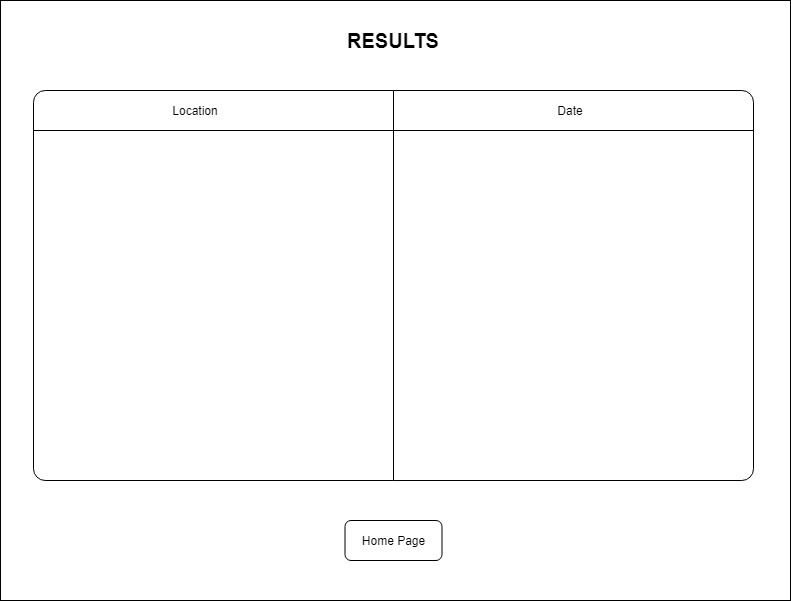
\includegraphics[width=\textwidth]{./images/diagrams/Charts} 
\caption{Results Page Mockup}
\label{fig:mockup}
\end{figure}

\clearpage

\section{Analysis and workflow}

% ----- REQUIREMENTS -----
\subsection{Requirements}

\subsubsection{Functional requirement}
The system has to allow the user to carry out basic functions such as:
\begin{itemize}
\item To start the text analysis.
\item To stop the text analysis.
\item To view the most recent recognized earthquakes from the application.
\end{itemize}
\vspace{2mm}
The system has to iteratively perform the following operations: 
\begin{itemize}
\item Real-time fetching of tweets.
\item Perform a classification of the tweets and obtain the label (earthquake or non-earthquake).
\item When an earthquake tweet is regocnized send a warning message.
\item When an earthquake tweet trend is recognized send an emergency message and add the relative earthquake information into the database.
\end{itemize}
\vspace{2mm}

\subsubsection{Non-functional requirements}
\begin{itemize}
\item Usability, ease of use and intuitiveness of the application by the user.
\item The system should provide a high level of accuracy.
\end{itemize}

\clearpage

% ----- USE CASES -----
\subsection{Use Cases}

\textbf{Actors}
\begin{itemize}
\item{User: this actor represents a user of the application}
\item{System: this actor represent the system}
\item{Twitter: this actor represent the Twitter service}
\end{itemize}

\subsubsection{Use Cases Description}
\begin{itemize}
\item Twitt Search : This use case can be performed by the user to start the real-time tweets fetching.
\item Retrive Tweet: This use case represents the action of getting a tweet from twitter.
\item Twitter Connection: This use case represents the connection with the Twitter service.
\item HTTP Request for Connection: This use case represents the Request for the connection to the Twitter Service.
\item HTTP Response for Connection: This use case represents the Response for the connection from the Twitter Service.
\item HTTP Request for Tweets: This use case represents the Request for tweets to the Twitter service.
\item HTTP Response for tweets: This use case represents the Response for tweets from the Twitter service.
\item Perform Text Analysis: This use case represents the process of Text analysis performed by the system.
\item Apply Classification Algorithm: This use case represents the classification of the tweets performed with the previously generated classifier by the "Generate Classifier" use case.
\item Show Warning Message: This use case displays an warning message if a few earthquake tweet are recognized.
\item Show Emergency Message: This use case displays an emergency message if a some earthquake tweet are recognized.
\item Add Earthquake To Database: This use case represent the insert of the recognized earthquake into the database.
\item Display Results: This use case shows the results of the classification.
\item Browse earthquakes: The system browses the earthquakes on the database.
\item Find earthquake: The system selects an earthquake on the database.
\item Display Earthquake: This use case shows the earthquake on the application.
\item Generate Classifier: This use case is performed automatically by the system and it generates a classifier using a training set. 
\item Browse Tweets: The system browses the tweets on the trainig dataset.
\item Train the classifier: Perform an algorithm to generate the classifier.
\item Stop Real-Time fetching: This use case allows the user to stop the real-time tweets fetching.
\end{itemize}

\begin{minipage}{\linewidth}
\begin{center}
\vspace{8mm}
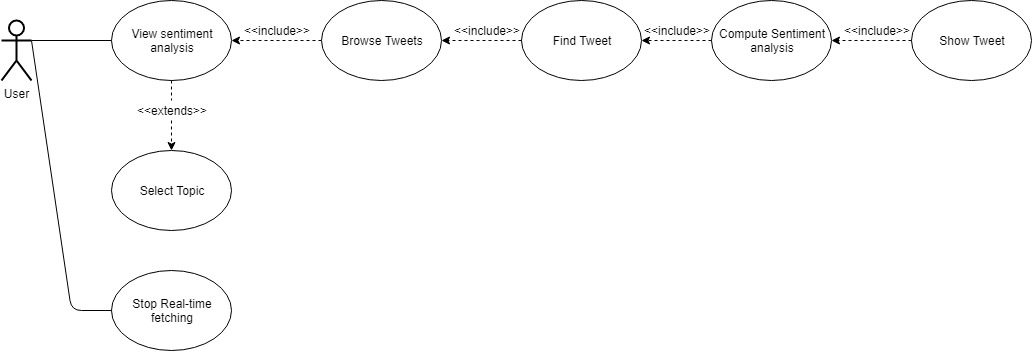
\includegraphics[ width=0.55\textheight]{./images/diagrams/UseCase} 
\captionof{figure}{Use cases diagram}
\vspace{3mm}
\end{center}
\end{minipage}


\clearpage
\subsection{System Flow Diagram}
\begin{minipage}{\linewidth}
\begin{center}
\vspace{8mm}
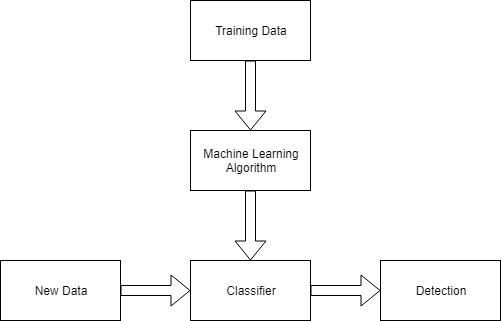
\includegraphics[ width=0.6\textheight]{./images/diagrams/Flow Diagram} 
\captionof{figure}{Flow Diagram}
\vspace{3mm}
\end{center}
\end{minipage}

\clearpage
\subsection{Text analysis process}
\begin{minipage}{\linewidth}
\begin{center}
\vspace{8mm}
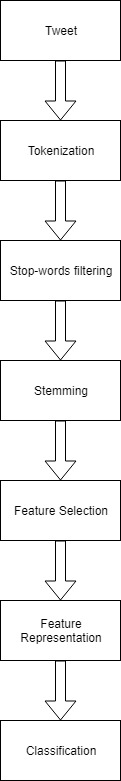
\includegraphics[ width=0.13\textheight]{./images/diagrams/Process} 
\captionof{figure}{Text Analysis Process}
\vspace{3mm}
\end{center}
\end{minipage}


\clearpage
\subsection{Analysis of entities}
This diagram represents the main entities of the application and the relations between them.
\begin{minipage}{\linewidth}
\begin{center}
\vspace{4mm}
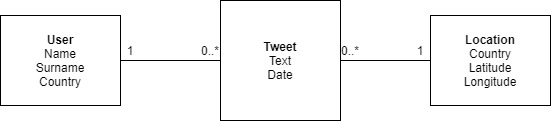
\includegraphics[width = 1\textwidth]{./images/diagrams/Uml Analysis diagram} 
\vspace{2mm}
\captionof{figure}{UML analysis diagram}
\label{fig:useCases}
\end{center}
\end{minipage}

\clearpage
\subsection{Data analysis}
\subsubsection{Building the classifier}
In order to build our classifier raw tweets have been scraped using a twitter scraping tool called Twint written in Python. Given location, tags to search for and a timestamp  (or a date interval), returns the informations about the tweets matching those parameters. For more information visit: \textcolor{blue}{\href{https://www.github.com/twintproject/twint}{Twint Github Page}}. To build the training set two different queries have been used: 
\begin{itemize}
\item The first query selects the tweets in Italy matching the tag {\#}terremoto.
\item The second query selects the tweets in Italy without tags.
\end{itemize} 
After that the labels (earthquake, non-earthquake) have been added manually to obtain a good training (and test) set to generate a classifier. We ended up with a balanced dataset of 300 tweets per class, 600 labeled tweets.\\
The training data will be stored in an arff file, after cleaning the text of the tweet. The second query is necessary to obtain better results because without the tweets obtained from it the classifier would suffer from overfitting.\\
Once the training data is ready a classification algorithm is applied in order to build the classifier.

\subsubsection{2016-2017 earthquakes database}
Another database was created by collecting (in the same way) tweets between the dates 2017-06-30 and 2016-06-01. With that database we managed to create an histogram to check if there are spikes of tweets corresponding to catastrofic earthquakes in order to perform an analysis. The total number of analyised tweets is 304307.

<histogram image>

As we can see there are 3 major spikes relative to the 24-08-2016, 30-10-2016 and 18-01-2017 huge earthquakes. We created the same histogram after performing a classification on the tweets using the classifier obtained from the training set.

\subsubsection{Application parameters}
Two parameters are used in this application:
\begin{itemize}
\item Number of tweets classified as "earthquake" to detect before sending a warning message.
\item Number of tweets classified as "earthquake" to detect before sending an emergency message.
\end{itemize}
We tested how many earthquake tweets are detected in a time span of 10 minutes of a real earthquake, then checked the same number for a random time span of 10 minutes. we obtained  5 tweets in 10 minutes for the 2016-10-30 and 0 tweets in a random date. We heuristically decided to put the first parameter at 2 and the second at 4.

\clearpage
\subsection{Model analysis}
\subsubsection{Choosing the classifier}
The choice of the classifier has been made by evaluating some quality measures of different classifiers applying a 10-fold cross-validation to find the best one for our application. A matrix of the results obtained from the different classifiers is show in the figure below.

<different classifiers measures>

The confusion matrix obtained from the classification is the following:

<confusion matrix of the classifier>

The SVM classifier seems to be the best for this application in terms of good accuracy and speed.



\clearpage
% ----- DESIGN -----
\section{Design}

\subsection{Software architecture}
The application is designed over 3 different layers, see figure \ref{fig:architecture_diagram}:
\begin{itemize}
\item Front-end
\item Middleware
\item Back-end
\end{itemize}
\vspace{5mm}
\begin{minipage}{\linewidth}
\begin{center}
\vspace{1mm}
\includegraphics[height = 100mm]{./images/diagrams/architecture} 
\vspace{6mm}
\captionof{figure}{Software architecture diagram\\}
\label{fig:architecture_diagram}
\end{center}
\end{minipage}
\vspace{7mm}
\clearpage


\clearpage
% ----- IMPLEMENTATION -----
\section{Implementation}
\subsection{Used technologies}
The application is developed in java programming language, version 11.0.4, and in JavaFX system to create the GUI, version 11, so it should run on each platform in which JVM is installed, but the application is tested and guardantee on Ubuntu 16 and Window OS. Moreover Maven is used  to build and mantain the project, version 3.8.0. \\
The java driver for mongo manage the comunication between client application layer and mongo backend layer, version 3.11.2.\\ 
For the background layer it is used Apache as web-server, version 2.4 (including MySql).\\
So this application is tested using these technologies, considering these particular versions: for other versions the correct execution isn't guaranteed .\\

\subsection{Declaration of class Tweet}
The following java-code shows a declaration of the class Tweet.
\vspace{2mm}
\\ <code here>
\vspace{5mm}

\noindent Another foundamental class is SQLManager, that manages the db-connection and the related operations.

\subsection{Building the classifier}
The following java-code shows the training part of the process to obtain our classifier using the SVM classification method.

<code here>


\subsection{Create}
Adding a tweet to the database.
\vspace{2mm}
 \\<Code here>
\vspace{5mm}

\subsection{Read}
This functionality returns a list of tweets.
\vspace{2mm}
\\<code here>
\vspace{5mm}

\subsection{Classification of a tweet}
This functionality performs a classification of a tweet.
\vspace{2mm}
\\<code here>
\vspace{5mm}

\clearpage

\subsection{GUI}
There is an fxml documents which describes the objects showed in the GUI interface of the  page.
\begin{itemize}
\item Home.fxml
\end{itemize}
In addiction there is a class, called Controller, that is in charge of handling events of the objects defined in the associated fxml document.
\begin{itemize}
\item HomeController.java
\end{itemize}

\clearpage
% MANUAL%
\section{User Manual}


\end{document}
